\documentclass[12pt, a4paper]{article}
\usepackage{amsmath, amssymb, mathrsfs}
\usepackage{graphicx}
\usepackage{url}
\usepackage{natbib}
\usepackage[margin=1in]{geometry}
\usepackage{braket}
\usepackage{bm}
\usepackage{tikz}
\usetikzlibrary{arrows.meta, decorations.pathmorphing, shapes.geometric, positioning}

\begin{document}

% Reactor Core Blueprint
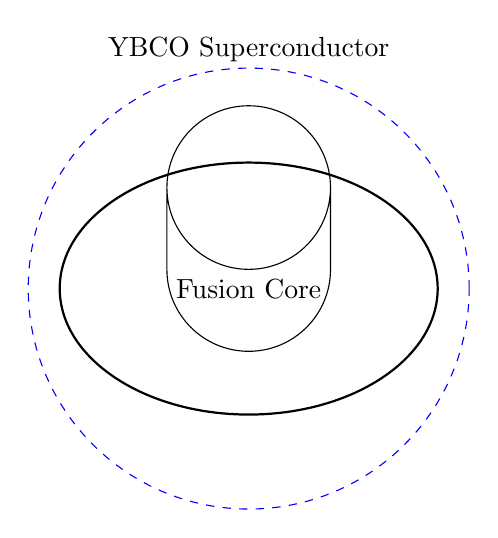
\begin{tikzpicture}[scale=0.8]
\draw[thick, ->] (0,0) circle [x radius=3cm, y radius=2cm];
\node[draw, cylinder, shape border rotate=90, minimum height=2cm] at (0,0) {Fusion Core};
\draw[dashed, blue] (0,0) circle [radius=3.5cm];
\node at (0,3.8) {YBCO Superconductor};
\end{tikzpicture}


\bibliographystyle{plainnat}
\bibliography{references}
\end{document}
